\section{Advanced Counting}
\subsection{Generating permutations}
There are situations in which it is necessary to generate, not just count, all permutations of a set or subsets of a given size.

\subsubsection*{Lexicographic Order}
A well-defined order imposed on the n-tuples is useful to systematically generate all the elements in a set of n-tuples. Generating the n-tuples in the set from smallest to largest ensures that each n-tuple is generated exactly once.

\bld{Lexicographic order} is a way or ordering n-tuples in which two n-tuples are compared according to the first entry where they differ. An example of such ordering is the word in a dictionary.

\subsubsection*{Generating Permutations}
A \bld{permutation} of the set $\{1,2,\ldots,n\}$ is an ordered n-tuple in which each number in $\{1,2,\ldots,n\}$ appears exactly once. For example, $(2,5,1,4,3)$ is a permutation of the set $\{1,2,3,4,5\}$.

\subsubsection*{Generating r-subsets of a set}
Unlike sequences or n-tuples, the order in which the elements of a set or subset are written does not matter. Sets can be ordered lexicographically by first sorting the elements in increasing order and then comparing the two sets as if they were ordered sequences. For example, $\{2,3,11\} < \{2,5,6\}$, because the first element is the same in both sets but in the second element $3 < 5$.

\subsection{Binomial coefficients and combinatorial identities}
An \bld{identity} is a theorem stating that two mathematical expressions are equal.

\subsubsection*{Theorem: A Simple Combinatorial Identity}
For any non-negative integers $n \tand k \tsuchthat k \leq n$:
\[
  \binom{n}{k} = \binom{n}{n-k}
\]

A proof that makes use of counting principles is called a \bld{combinatorial proof}. Combinatorial proofs usually involve defining a set $S$ and counting the number of elements in $S$ to get a mathematical expression for the number of items in the set. Every combinatorial proof of an identity uses a bijection implicitly as part of the argument.

\subsubsection*{Theorem: The Binomial Theorem}
For any non-negative integer $n$ and any real numbers $a \tand b$:
\[
  (a + b)^n = \sum_{k=0}^{n} \binom{n}{k} a^{n-k}b^k = \sum_{k=0}^{n} \binom{n}{k} a^kb^{n-k}
\]
The coefficients $\binom{n}{k}$ are called binomial coefficients.

For the case $n = 5$, the Binomial Theorem says that
\begin{align*}
  (a+b)^5 & = \binom{5}{0}a^5 + \binom{5}{1}a^4b + \binom{5}{2}a^3b^2 + \binom{5}{3}a^2b^3 + \binom{5}{4}ab^4 + \binom{5}{5}b^5 \\
          & = a^5 + 5a^4b + 10a^3b^2 + 10a^2b^3 + 5ab^4 + b^5
\end{align*}

The Binomial Theorem can also be used to obtain combinatorial identities. For example, by plugging in $a=b=1$, the Binomial Theorem yields the identity below.
\[
  2^n = \sum_{k=0}^{n} \binom{n}{k}
\]

Similarly, by letting $a=-1 \tand b=1$, and requiring that $n$ be positive, the left hand side of the Binomial Theorem becomes 0. The right hand side of the Binomial Theorem becomes:
\[
  0 = \sum_{k=0}^{n}(-1)^k \binom{n}{k}
\]
In the expanded form,
\[
  \binom{n}{0} - \binom{n}{1} + \binom{n}{2} - \binom{n}{3} + \cdots + (-1)^n \binom{n}{n} = 0
\]

\subsubsection*{Pascal's Triangle}
The $17^{th}$ century French mathematician, Blaise Pascal, developed a triangular chart that contains all the number of the form $\binom{n}{k}$. The chart, now known as Pascal's Triangle, can be used to derive the value of a particular $\binom{n}{k}$. The $n^{th}$ row of Pascal's Triangle contains the $n+1$ binomial coefficients of the form $\binom{n}{k}$ as shown in the figure below.
\[
  \begin{array}{cccccccccc}
    n=0 &              &              &              &              & \binom{0}{0} &              &              &                             \\
    n=1 &              &              &              & \binom{1}{0} &              & \binom{1}{1} &              &                             \\
    n=2 &              &              & \binom{2}{0} &              & \binom{2}{1} &              & \binom{2}{2} &                             \\
    n=3 &              & \binom{3}{0} &              & \binom{3}{1} &              & \binom{3}{2} &              & \binom{3}{3}                \\
    n=4 & \binom{4}{0} &              & \binom{4}{1} &              & \binom{4}{2} &              & \binom{4}{3} &              & \binom{4}{4} \\
  \end{array}
\]

\subsubsection*{Theorem: Pascal's Identity}
For any positive $n \tand k \tsuchthat k < n$:
\[
  \binom{n}{k} = \binom{n-1}{k-1} + \binom{n-1}{k}
\]

\subsection{The pigeonhole principle}
The pigeonhole principle is a mathematical tool used to establish that repetitions are guaranteed to occur in certain sets and sequences. The \bld{pigeonhole principle} says that if $n+1$ pigeons are placed in $n$ boxes, then there must be at least one box with more than one pigeon. The diagram below shows 10 pigeons, represented as $P$, in 9 boxes.
\begin{center}
  \begin{tabular}{ccc}
    $P$ & $P$ & $P$   \\
    $P$ & $P$ & $P,P$ \\
    $P$ & $P$ & $P$
  \end{tabular}
\end{center}

\subsubsection*{Theorem: The Pigeonhole Principle}
If a function $f$ has a domain of size at least $n+1$ and a target of size at most $n$, where $n$ is a positive integer, then there are two elements in the domain that map to the same element in the target (i.e., the function is not one-to-one)

\subsubsection*{Theorem: The Generalized Pigeonhole Principle}
Consider a function whose domain has at least $n$ elements and whose target has $k$ elements, for $n \tand k$ positive integers. Then there is an element $y$ in the target such that $f$ maps at least $\lceil n/k \rceil$ elements in the domain to $y$.

\subsubsection*{Theorem: Converse of the Generalized Pigeonhole Principle}
Suppose that a function $f$ maps a set of $n$ elements to a target with $k$ elements, where $n \tand k$ are positive integers. In order to guarantee that there is an element $y$ in the target to which $f$ maps to at least $b$ elements from the domain, then $n$ must be at least $k(b-1)+1$.

\subsection{Generating functions}
Generating functions are a powerful tool that can be used to solve a variety of problems related to counting and recurrence relations. A \bld{generating function} is a way of representing a sequence of number as a n algebraic function in which each term in the sequence is a coefficient of an $x^j$ term in the function. The advantage of representing sequences algebraically is that there are many techniques from algebra that can be used to manipulate functions which then leads to insight about the sequences they represent.

The sequence $f_0,f_1,f_2,f_3,\ldots$ is represented by the generating function
\[
  F(x) = f_0 + f_1x + f_2x^2 + f_3x^3 + \cdots
\]

The numbers in the sequence are the coefficients of the terms in $F(x)$. For the sequence $1,1,1,1,\ldots$ is represented by the generating function
\[
  H(x) = 1 + x + x^2 + x^3 + \cdots
\]
When $|x|<1$ for $H(x)$ the sum is finite and has a closed form of
\[
  H(x) = \sum_{j=0}^{\infty} x^j = \frac{1}{1-x}
\]
Additionally, for the partial sum up to $x^k$,
\[
  \sum_{j=0}^{k} x^j = \frac{1-x^k}{1-x}
\]

\subsubsection*{Using Generating Functions for Counting}
One of the primary uses for generating functions is to help solve counting problems. In general, $f_j$ is the number of way to select a subset of $j$ objects.

Consider the situation in which there is a set of two apples and one banana. The apples are indistinguishable, so selecting one apple is the same as selecting the other.
\begin{center}
  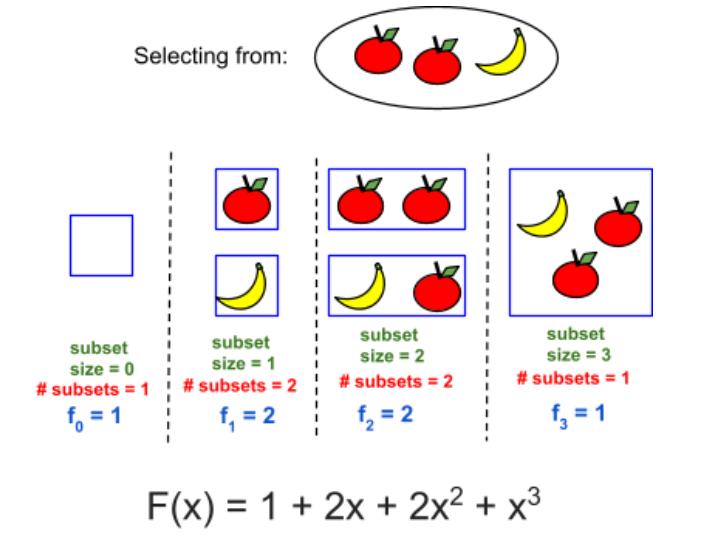
\includegraphics[width=.6\linewidth]{resources/11_two_apple_one_banana.png}
\end{center}

If the set from which the subsets are selected is an infinite set, then the resulting sequence is also infinite.

\subsubsection*{Summary of Generating Functions}
\begin{center}
  \begin{tabular}{|c|c|c|}
    \hline
    Description                                                  & Long Form                            & Short Form                               \\
    \hline
    Infinite supply of one kind of item                          & $1 + x + x^2 + x^3 + \cdots$         & ${\displaystyle \frac{1}{1-x}}$          \\
    \hline
    Selecting from a set of $n$ identical items                  & $1 + x + x^2 + x^3 + \cdots + x^n$   & ${\displaystyle \frac{1-x^{n-1}}{1-x}}$. \\
    \hline
    Infinite supple of identical items grouped in batches of $k$ & $1 + x^k + x^{2k} + x^{3k} + \cdots$ & ${\displaystyle \frac{1}{1-x^k}}$        \\
    \hline
    Infinite supple of 2 different kinds of items                & $1 + 2x + 3x^2 + 4x^3 + \cdots$      & ${\displaystyle \frac{1}{(1-x)^2}}$      \\
    \hline
  \end{tabular}
\end{center}

\subsubsection*{Products of Generating Functions}
Generating functions become very useful when different sets of objects are combined together into larger sets.

For example, if we are selecting subsets of apples from a set of 3 apples, the generating function is $A(x) = 1 + x + x^2 + x^3$, and if we are selecting bananas from a set of 2 bananas, the generating function is $B(x) = 1 + x + x^2$. Now suppose we pool the three apples and two bananas into a set of five pieces of fruit and ask 'how many ways can one select a set of fruit from the collection of five pieces of fruit?'

The power of generating functions is illustrated in the fact that if we take the product of $A(x)$, the generating function for apples, and $B(x)$, the generating function for bananas, to get $A(x)B(x)$, then the resulting product is the generating function for the pooled set of five pieces.
\[
  A(x)B(x) = (1 + x + x^2 + x^3)(1 + x + x^2) = 1 + 2x + 3x^2 + 3x^3 + 2x^4 + x^5
\]
Note that the rule of multiplying generating function only works when the two sets of objects being combined are \itl{distinct}. The rule would not work for combining two sets of indistinguishable apples.

Now suppose that we add oranges to the set of selections. There are three oranges, but they come wrapped in a single pack, so one can select zero or three oranges, but not one or two. The generating function for oranges is $O(x) = 1 + x^3$. Again, we can take the product of the generating functions to solve, 'how many ways are there to select subsets of fruit of a particular size?'
\[
  A(x)B(x)O(x) = 1 + 2x + 3x^2 + 4x^3 + 4x^4 + 4x^5 + 3x^6 + 2x^7 + x^8
\]
The coefficient of $x^5$ in the generating function for the whole set of fruit is 4, so there are 4 ways to select 5 pieces of fruit.